\documentclass{standalone}
\usepackage{tikz}
\usepackage{tikz-feynman} % Paquete para diagramas de Feynman
\usepackage{amsmath} % Para el símbolo de la llave

\begin{document}

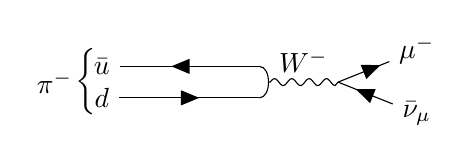
\begin{tikzpicture}
    \begin{feynman}
        % Nodos de partículas con posiciones ajustadas
        \vertex (iu) at (0,1) {$\Bar{u}$}; % No cambia, ya que x=0
        \vertex (fu) at (2,1);       % x = 3 - 1
        \vertex (id) at (0,0.6) {$d$}; % No cambia, ya que x=0
        \vertex (fd) at (2,0.6);     % x = 3 - 1
        \vertex (iw) at (2.12,0.8);  % x = 3.12 - 1
        \vertex (fw) at (3,0.8);     % x = 4 - 1
        \vertex (imu) at (4,1.2){$\mu^-$}; % x = 5 - 1
        \vertex (inu) at (4,0.4){$\bar{\nu}_\mu$}; % x = 5 - 1
        % Nodo para la llave
        \node[left] at (-0.25,0.8){$\pi^-$};
        \node[] at (0,0.8) {\(\left\{\begin{array}{c} \\\\ \end{array} \right.\)};

        % Diagramas de líneas
        \diagram* {
            % Líneas del pión
            (iu) --[anti fermion] (fu),
            (id) --[fermion] (fd),
            (fu) -- [out=0, in=0] (fd),
            % Línea del W+
            (iw) -- [boson, edge label=$W^-$] (fw),
            % Líneas leptónicas
            (imu) --[anti fermion] (fw),
            (inu) --[fermion] (fw),
        };
        
    \end{feynman}
\end{tikzpicture}

\end{document}
